PanDA consists of several interconnected subsystems, most of them are built from off-the-shelf and Open Source components. Figure \ref{fig:architecture} shows a schematic view of the PanDA system.
In the following we will briefly describe system’s architecture and components.

\begin{itemize}
\item PanDA Server
\item Pilot
\item Factory
\item PanDA monitoring
\item JEDI ??
\item What else?
\end{itemize}

\begin{figure}
\begin{center}
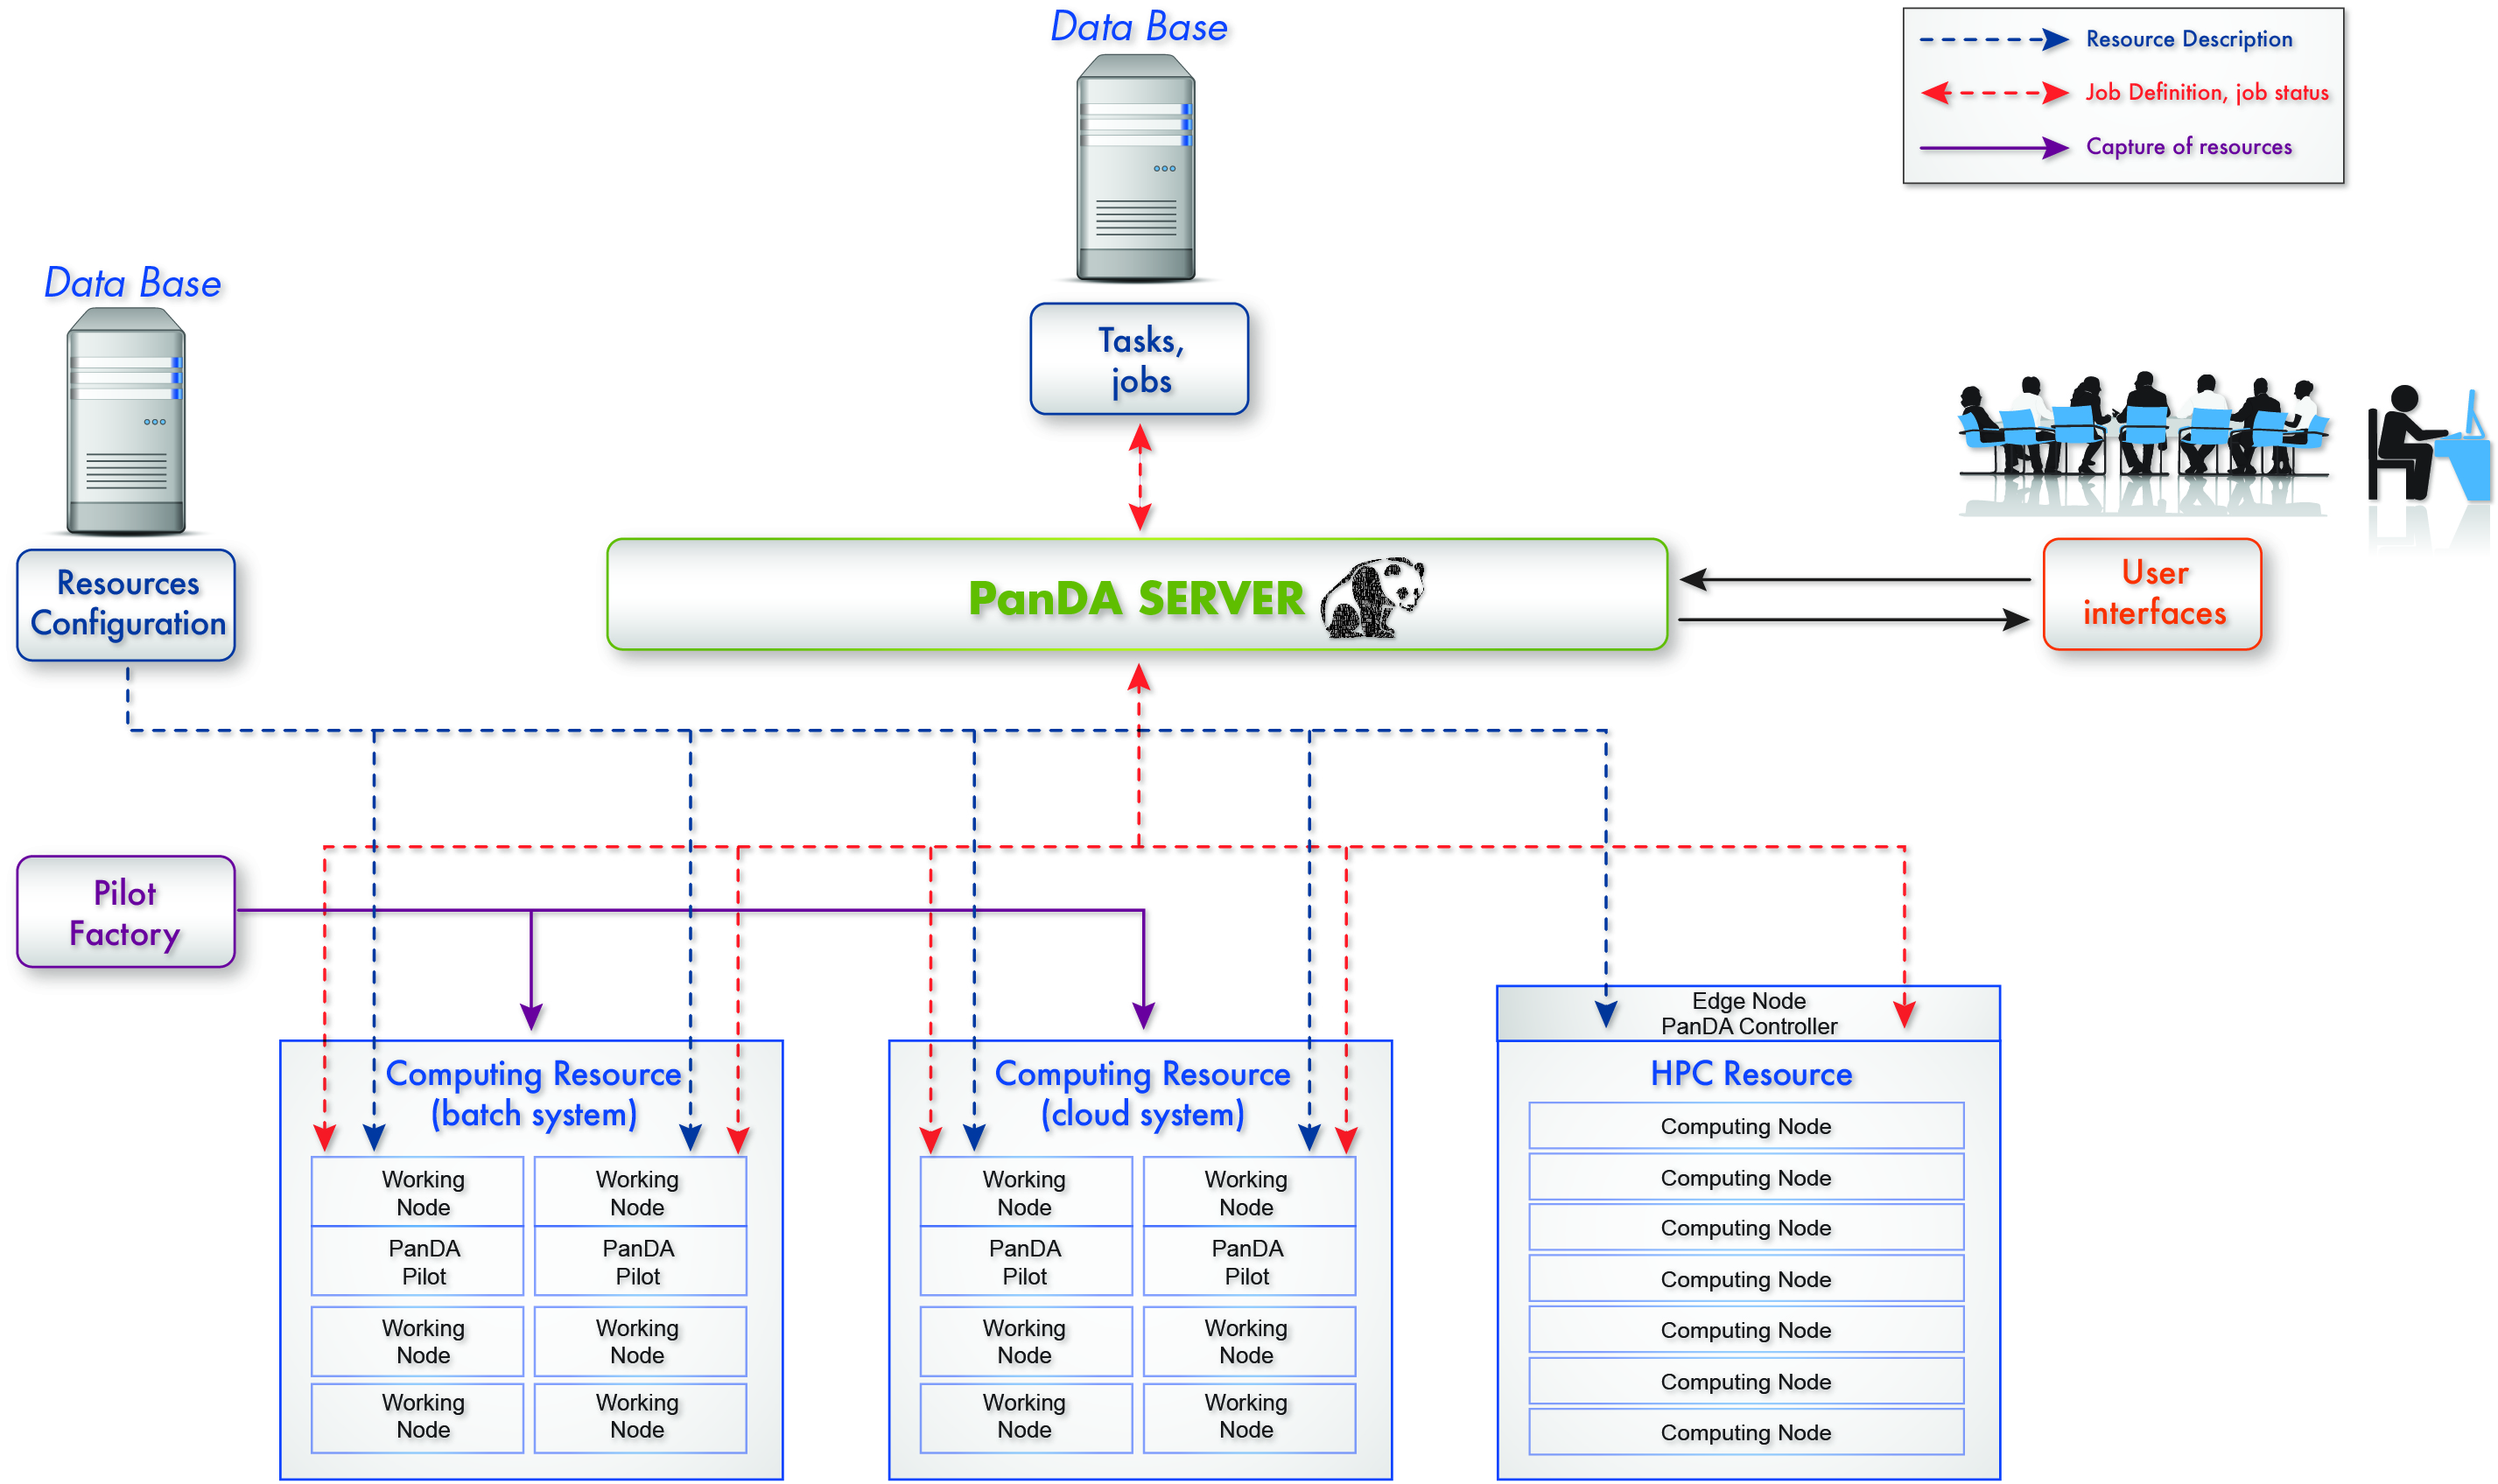
\includegraphics[width=\columnwidth]{figures/PandaArch.jpg}
\caption{Schematic view of the PanDA system\label{fig:architecture}. 
  Originally PanDA was designed for grid infrastructure... In this paper
  is focussed on the HPC use case; there are differences from  the grid use
  case. This paper discusses how PanDA has been adapted to execute a workload on
  HPC resources. The schematic overview is presented for workload X on Titan......}
\end{center}
\end{figure}
\subsection{PanDA Server}
The PanDA server is the main component of the system, It provides  a task queue managing all job information centrally. The PanDA  server receives jobs through the client interface into the task queue, upon which a brokerage module  operates to prioritize  and assign work on the basis of job type, priority, input data and its locality, and available CPU resources. The PanDA  server operates as a web service. It runs on Apache web server, interacting with the back-end database running  on separate servers. It uses the Apache worker  model, with many independent   processes  handling client requests  in  parallel. Since all  state is maintained  in  the central database,  the PanDA Server application instance itself is stateless. Currently production version of PanDA utilizes Oracle database backend, but PanDA  can also work with MySQL family of databases.

\subsection{PanDA Pilot}
 PanDA is a pilot based workload  management system. In the PanDA job lifecycle, pilot jobs (Python scripts that organize workload processing on a worker  node) are submitted to sites. When these  pilot jobs start on a  worker node they contact a central  server  to retrieve  a real payload (i.e., an end-user job) and execute it. Using these pilot-based  workflows helps to improve job reliability, optimize resource utilization, allows for opportunistic  resources usage, and mitigates  many of the problems  associated with the inhomogeneities found on the Grid.
The pilots themselves  do not contain all the functionality needed to request a payload  job from the Panda Server. First, the complete  set of pilot code is downloaded via HTTP from a  central Subversion repository.  The repository works with Apache web server configured  with a  memory-based   web proxy (Squid). The purpose  of the cache  is to reduce  the request load on the back-end Subversion  server. That allows for a  very good performance since only occasional  queries trigger a  full  lookup on the back-end  Subversion  system, and most external  queries are pulled from memory on the front-end web server. The benefits of this system include a high-performance code download service combined with code updates still being immediately  available  as soon as they are committed to source code control.

\subsection{PanDA Factory}
As a pilot-based  system, PanDA  requires some way to get the initial PanDA pilot onto worker nodes at sites. This is done with the help of a component  called AutoPyFactory (APF). APF runs in a single daemonized process, launching  a separate thread for each internal  workflow. Each one of these internal workflows typically serves  a single job queue  as defined  in WMS, and delivers pilots to a single batch queue, either local or remote. The behavior of these APF workflows is determined by the combination of a set  of plugins, invoked in a  fixed order, in a loop, each one in charge of the performance of a well defined action.

\subsection{PanDA Monitoring}
The PanDA Monitor is a web-based dashboard-style  graphical application. It runs on Apache and interacts with the back-end database for persistence. The Monitor is the primary way that users and site administrators get a  view into the status of current and past jobs, data movement,  pilot factory. The Monitor allows users  access  to all job log files on job by job basis thus greatly simplifying code debugging and failure analysis in distributed computing environment.






